\documentclass[12pt]{article}

\usepackage{graphicx}
\usepackage{paralist}
\usepackage{amsfonts}
\usepackage{amsmath}
\usepackage{hhline}
\usepackage{booktabs}
\usepackage{multirow}
\usepackage{multicol}
\usepackage{url}

\oddsidemargin -10mm
\evensidemargin -10mm
\textwidth 160mm
\textheight 200mm
\renewcommand\baselinestretch{1.0}

\pagestyle {plain}
\pagenumbering{arabic}

\newcounter{stepnum}

%% Comments

\usepackage{color}

\newif\ifcomments\commentstrue

\ifcomments
\newcommand{\authornote}[3]{\textcolor{#1}{[#3 ---#2]}}
\newcommand{\todo}[1]{\textcolor{red}{[TODO: #1]}}
\else
\newcommand{\authornote}[3]{}
\newcommand{\todo}[1]{}
\fi

\newcommand{\wss}[1]{\authornote{blue}{SS}{#1}}

\title{Assignment 4, Design Specification}
\author{SFWRENG 2AA4}

\begin{document}

\maketitle
The following Module Interface Specification outlines the necessary modules and their respective access routine programs, state variables, and local functions required for implementing the popular web/mobile game $2048$. Players manipulate a 4x4 board that consists of randomly spawned tiles, and combine tiles with equal values into greater powers of two, until either the 2048 tile is reached or the player runs out of possible moves.

\medskip

An example of the game being modelled in this design specification can be found on the website https://play2048.co/

\begin{center}
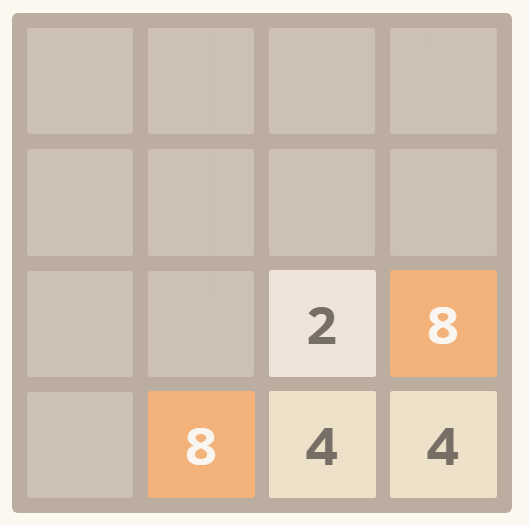
\includegraphics[width=0.5\textwidth]{images/2048game.png}
\end{center}

\newpage

\subsection*{Changes my design considers or design changes in the future:}

\begin{itemize}
  \item Using Java UI libraries to display the board in a more user friendly way.
  \item Further generalize the board, make it more modular (i.e. allowing the ability to change dimension of the board during runtime).
  \item Take in user input via keyboard or mouse, rather than typing the actual direction the user wants the board to move.
\end{itemize}

\newpage

\section{Informal Design Overview}

The design outlined in this specification adheres to the MVC design. The model, in this case, is the Game module itself. The Game module has direct access to the Board module and is managed by it. The module is directly updated and modified by the controller, and all aspects of the game is managed by this module. The view portion of the MVC design is the TextInterface module, which is accessible by the module's \verb|getInstance()| function, and is updated by the controller and prints out any necessary messages to the user, including, but not limited to, the end messages and the end score. Finally, the controller is the GameState module, which inherits a State abstract module. Modules that inherit State repeatedly run its \verb|execute| function until the State child exits the state, which serves as the basis for the controller's functionality. In terms of the GameState module, a child of the State abstract module, the GameState's \verb|execute| functionality consists of taking in user input, as well as manipulating the Game module accordingly, depending on the user input. It checks repeatedly if the game is in progress, and if it is not, it exits the state and enters the \verb|WinState| or \verb|LoseState| accordingly.

\newpage

\noindent To further visualize how the program runs and behaves, a UML diagram can be seen below:

\begin{center}
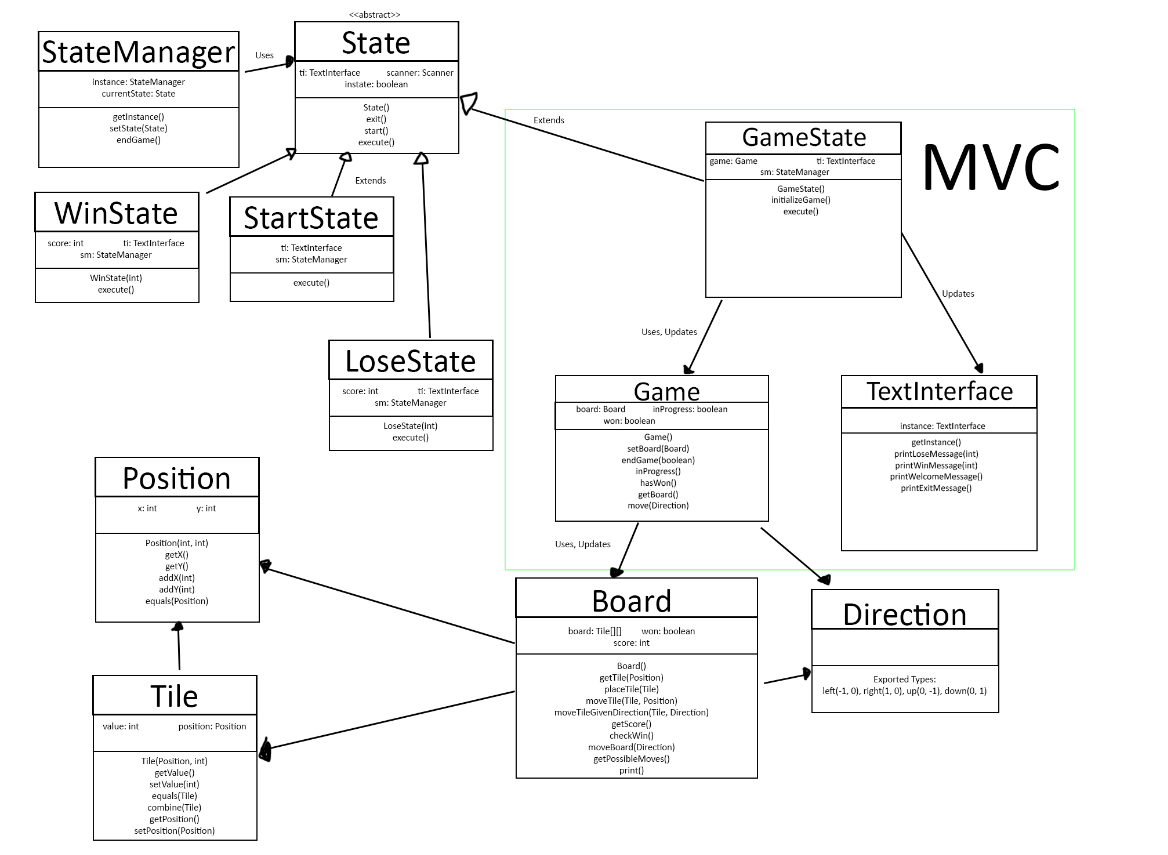
\includegraphics[width=1\textwidth]{images/uml.png}
\end{center}

As can be seen in the UML diagram, the MVC consists of the Game (model), TextInterface (view), and GameState (controller). The State system can be seen in the top left, with the WinState, StartState, and LoseState all being children of the State abstract module. The Game module manipulates the Board module, updating it depending on the user input that is provided by the controller GameState module.

\medskip

\newpage

\section* {Direction Module}

\subsection*{Module}

Direction

\subsection* {Uses}

N/A

\subsection* {Syntax}

\subsubsection* {Exported Constants}

None

\subsubsection* {Exported Types}

Direction = \{left, right, up, down\}

\medskip

\subsubsection* {Exported Access Programs}

None

\subsection* {Semantics}

\subsubsection* {State Variables}

None

\subsubsection* {State Invariant}

None

\newpage

\section* {Position ADT Module}

\subsection* {Template Module}

Position

\subsection* {Uses}

None

\subsection* {Syntax}

\subsubsection* {Exported Types}

None

\subsubsection* {Exported Access Programs}

\begin{tabular}{| l | l | l | l |}
\hline
\textbf{Routine name} & \textbf{In} & \textbf{Out} & \textbf{Exceptions}\\
\hline
Position & $\mathbb{N}, \mathbb{N}$ & Position & ~ \\
\hline
getX & ~ & $\mathbb{N}$ & \\
\hline
getY & ~ & $\mathbb{N}$ & \\
\hline
addX & $\mathbb{N}$ & ~ & ~ \\
\hline
addY & $\mathbb{N}$ & ~ & ~ \\
\hline
equals & Position & $\mathbb{B}$ & ~\\
\hline
\end{tabular}

\subsection* {Semantics}

\subsubsection* {State Variables}

x: $\mathbb{N}$\\
y: $\mathbb{N}$\\

\subsubsection* {State Invariant}

$x >= 0 \land x <= 3 \land y >= 0 \land y <= 3$

\subsubsection* {Assumptions}

None

\subsubsection* {Access Routine Semantics}

\noindent Position($xPos, yPos$):
\begin{itemize}
\item transition: x, y $:=$ $xPos$, $yPos$
\item output: $out := \mathit{self}$
\end{itemize}

\noindent getX():
\begin{itemize}
\item transition: none
\item output: $out := $ x
\end{itemize}

\noindent getY():
\begin{itemize}
\item transition: none
\item output: $out := $ y
\end{itemize}

\noindent addX($xPos$):
\begin{itemize}
\item transition: x $:=$ x $+$ $xPos$
\item output: none
\end{itemize}

\noindent addY($yPos$):
\begin{itemize}
\item transition: y $:=$ y $+$ $yPos$
\item output: none
\end{itemize}

\noindent equals($p$):
\begin{itemize}
\item transition: none
\item output: $out := $ (getX() $=$ p.getX() $\land$ getY() $=$ p.getY())
\end{itemize}

\subsubsection* {Local Functions}

constrainXPos: void $\rightarrow$ void\\
constrainXPos() $\equiv$ $((x < 0) \Rightarrow x = 0) \land ((x > 3) \Rightarrow x = 3)$\\

\noindent constrainYPos: void $\rightarrow$ void\\
constrainYPos() $\equiv$ $((y < 0) \Rightarrow y = 0) \land ((y > 3) \Rightarrow y = 3)$\\

\newpage

\section* {TextInterface Module}

\subsection* {Module}

UserInterface

\subsection* {Uses}

None

\subsection* {Syntax}

\subsubsection* {Exported Constants}

None

\subsubsection* {Exported Types}

None

\medskip

\subsubsection* {Exported Access Programs}

\begin{tabular}{| l | l | l | p{6cm} |}
\hline
\textbf{Routine name} & \textbf{In} & \textbf{Out} & \textbf{Exceptions}\\
\hline
getInstance & ~ & TextInterface &  \\
\hline
printLoseMessage & $\mathbb{N}$ & ~ & \\
\hline
printWinMessage & $\mathbb{N}$ & ~ & \\
\hline
printWelcomeMessage & ~ & ~ & \\
\hline
printExitMessage & ~ & ~ & \\
\hline
\end{tabular}

\subsection* {Semantics}

\subsection*{Environment Variables}

window: Section of the computer screen to display the text interface.

\subsubsection* {State Variables}

instance: TextInterface

\subsubsection* {State Invariant}

None

\subsubsection* {Assumptions}

\begin{itemize}
\item Assume that each subroutine is called after the constructor has been called. The constructor can only be called once.
\end{itemize}

\subsubsection* {Access Routine Semantics}

\noindent getInstance():
\begin{itemize}
  \item transition: instance $:=$ (instance = null $\Rightarrow$ new TextInterface())
  \item output: \textit{self}
  \item exception: None
\end{itemize}

\noindent printLoseMessage($score$):
\begin{itemize}
\item transition: window $:=$ Print a message to the screen when the user loses the game, which displays the total score the user achieved. 
\end{itemize}

\noindent printWinMessage($score$):
\begin{itemize}
\item transition: window $:=$ Print a message to the screen when the user wins the game, which displays the total score the user achieved.
\end{itemize}

\noindent printWelcomeMessage():
\begin{itemize}
\item transition: window $:=$ Prints a welcome message when the user first launches the game.
\end{itemize}

\noindent printExitMessage():
\begin{itemize}
\item transition: window $:=$ Prints an exit message when the user exits the game.
\end{itemize}

\subsubsection*{Local Function:}

TextInterface: void $\rightarrow$ TextInterface \\
TextInterface() $\equiv$ new TextInterface()

\newpage

\section* {Tile ADT Module}

\subsection* {Template Module}

Tile

\subsection* {Uses}

None

\subsection* {Syntax}

\subsubsection* {Exported Types}

None

\subsubsection* {Exported Access Programs}

\begin{tabular}{| l | l | l | l |}
\hline
\textbf{Routine name} & \textbf{In} & \textbf{Out} & \textbf{Exceptions}\\
\hline
Tile & $Position, \mathbb{N}$ & Tile & \\
\hline
getValue & ~ & $\mathbb{N}$ & \\
\hline
setValue & $\mathbb{N}$ & ~ & \\
\hline
equals & Tile & $\mathbb{B}$ & ~\\
\hline
getPosition & ~ & Position & \\
\hline
setPosition & Position & ~ & \\
\hline
\end{tabular}

\subsection* {Semantics}

\subsubsection* {State Variables}

value: $\mathbb{N}$\\
position: Position\\

\subsubsection* {State Invariant}

None

\subsubsection* {Assumptions}

None

\subsubsection* {Access Routine Semantics}

\noindent Tile($p, val$):
\begin{itemize}
\item transition: value, position $:=$ $val$, p
\item output: $out := \mathit{self}$
\item exception: None
\end{itemize}

\noindent getValue():
\begin{itemize}
\item transition: none
\item output: $out := $ value
\end{itemize}

\noindent setValue($v$):
\begin{itemize}
\item transition: value $:=$ $v$
\item output: none
\end{itemize}

\noindent equals($tile$):
\begin{itemize}
\item transition: none
\item output: $out := $ value $\equiv$ tile.getValue()
\end{itemize}

\noindent getPosition():
\begin{itemize}
\item transition: none
\item output: $out := $ position
\end{itemize}

\noindent setPosition(newPos):
\begin{itemize}
\item transition: position $:=$ $newPos$
\item output: none
\end{itemize}

\newpage

\section* {State Abstract Module}

\subsection* {Abstract Module}

State

\subsection*{Uses}

TextInterface, Scanner

\subsection* {Syntax}

\subsection*{Exported Constants}

None

\subsection*{Exported Types}

None

\subsubsection* {Exported Access Programs}

\begin{tabular}{| l | l | l | p{6cm} |}
\hline
\textbf{Routine name} & \textbf{In} & \textbf{Out} & \textbf{Exceptions}\\
\hline
State & ~ & State & ~\\
\hline
exit & ~ & ~ & \\
\hline
start & ~ & ~ & \\
\hline
execute & ~ & ~ & \\
\hline
\end{tabular}

\subsection* {Semantics}

\subsection*{Environment Variables}

None

\subsubsection* {State Variables}

ti: TextInterface\\
scanner: Scanner\\
instate: $\mathbb{B}$\\

\subsubsection* {State Invariant}

None

\subsubsection* {Assumptions}

None

\subsubsection* {Access Routine Semantics}

\noindent new State():
\begin{itemize}
  \item transition: ti, scanner, instate $:=$ TextInterface.getInstance(), new Scanner(System.in), true
  \item output: \textit{self}
  \item exception: None
\end{itemize}

\noindent exit():
\begin{itemize}
\item transition: instate $:=$ false
\end{itemize}

\noindent start():
\begin{itemize}
\item transition: operational method that continuously runs the 'execute' abstract method until $instate$ state variable equals false.
\end{itemize}

\noindent execute():\\
This is an abstract function that is inherited by State children. As mentioned in the start() method semantics, this function will continuously update as long as the state is active.

\subsubsection*{Local Function:}

None

\newpage

\section* {StateManager Module}

\subsection* {Template Module}

StateManager

\subsection* {Uses}

State, TextInterface

\subsection* {Syntax}

\subsubsection* {Exported Types}

None

\subsubsection* {Exported Constant}

None

\subsubsection* {Exported Access Programs}

\begin{tabular}{| l | l | l | l |}
\hline
\textbf{Routine name} & \textbf{In} & \textbf{Out} & \textbf{Exceptions}\\
\hline
getInstance & ~ & StateManager & \\
\hline
setState & State & ~ & \\
\hline
endGame & ~ & ~ & \\
\hline
\end{tabular}

\subsection* {Semantics}

\subsubsection* {State Variables}

currentState: State\\
instance: StateManager\\
view: Area of window that displays text.\\

\subsubsection* {State Invariant}

None

\subsubsection* {Access Routine Semantics}

\noindent getInstance():
\begin{itemize}
\item transition: instance $:=$ (instance = null) $\Rightarrow$ new StateManager()
\item output: $out :=$ instance
\item exception: none
\end{itemize}

\noindent setState(state):
\begin{itemize}
\item transition: currentState $:=$ state$|$True $\Rightarrow$ currentState.start()
\item output: none
\item exception: none
\end{itemize}

\noindent endGame():
\begin{itemize}
\item transition: currentState, view $:=$ null, TextInterface.getInstance().printExitMessage()
\item output: none
\item exception: none
\end{itemize}

\newpage

\section* {Board ADT Module}

\subsection*{Template Module}

Board, Direction, Position

\subsection* {Uses}

Tile

\subsection* {Syntax}

\subsubsection* {Exported Types}

None

\subsubsection* {Exported Constant}

None

\subsubsection* {Exported Access Programs}

\begin{tabular}{| l | l | l | l |}
\hline
\textbf{Routine name} & \textbf{In} & \textbf{Out} & \textbf{Exceptions}\\
\hline
Board & ~ & Board & \\
\hline
getTile & Position & Tile & \\
\hline
placeTile & Tile & ~ & \\
\hline
moveTile & Tile, Position & ~ & ~\\
\hline
moveTileGivenDirection & Tile, Direction & ~ & \\
\hline
moveBoard  &  Direction  &  ~     & \\
\hline
getScore & ~ & $\mathbb{N}$ & ~\\
\hline
checkWin & ~ & $\mathbb{B}$ & ~\\
\hline
getPossibleMoves & ~ & $\mathbb{N}$ & ~\\
\hline
print & ~ & ~ & ~ \\
\hline
\end{tabular}

\subsection* {Semantics}

\subsection* {Environment Variables}

window: Section of the computer screen to display the game board.

\subsubsection* {State Variables}

board: sequence [4, 4] of Tile \\
won: $\mathbb{B}$\\
score: $\mathbb{N}$\\

\subsubsection* {State Invariant}

None

\subsubsection* {Assumptions}

\begin{itemize}
  \item Assume there is a random function that randomly generates a piece onto the board.
\end{itemize}

\subsubsection* {Design decision}

Coordinates of the board is represented as a 2D sequence. Each index of this sequence contains a Tile object.

\begin{center}
  In the above illustration, cell at (0,0) is stored in board[0][7].
\end{center}

\begin{itemize}
  \item The reasoning for this choice of data structure is how easy it is to get a tile at a specific point in the board. And since 2048 is essentially a two dimensional grid, it was obvious to use a two dimensional array to represent the game board.
\end{itemize}

\subsubsection* {Access Routine Semantics}

Board():
\begin{itemize}
\item transition: \\
      board $:=$ new Tile[4][4]\\
      generateRandomPiece(2)
\item output: $out := \mathit{self}$
\item exception: None
\end{itemize}

\noindent getTile(p):
\begin{itemize}
\item transition: none
\item output: $out :=$ board[p.getX()][p.getY()]
\item exception: None
\end{itemize}

\noindent placeTile(t):
\begin{itemize}
\item transition: board $:=$ \{tile : board$|$$tile \in board$ : (tile.getX() $=$ t.getX() $\land$ tile.getY() $=$ t.getY()) $\Rightarrow$ (tile $=$ t)\}
\item output: none
\item exception: None
\end{itemize}

\noindent moveTile(tile, p):
\begin{itemize}
\item transition: board $:=$ \{t : board$|$$t \in board$ : (tile.getX() $=$ t.getX() $\land$ tile.getY() $=$ t.getY()) $\Rightarrow$ (t $=$ null $\land$ placeTile(new Tile(p, tile.getValue())))\}
\item output: none
\item exception: none
\end{itemize}

\noindent moveTileGivenDirection(t, d):
\begin{itemize}
\item transition:\\ board $:=$ ((getTile(newPosition) $\neq$ null $\land$ tile $\neq$ t $\land$ t.equals(tile)) $\Rightarrow$ t.combine(tile) $\land$ score += t.getValue() $\land$ (t.getValue() = 2048 $\Rightarrow$ won $:=$ true))$|$True $\Rightarrow$ (moveTile(t, newPosition) $\land$ t.setPosition(newPosition))\\\\
where $newPosition$ $\equiv$ calculateFinalTilePosition(t, d) and $tile$ $\equiv$ getTile(newPosition)
\end{itemize}

\noindent moveBoard(d):
\begin{itemize}
\item transition: \{iterative : board$| iterative \in board : $\{t : iterative$|$ $t \in iterative : $ ((t $\neq$ null $\land$ canTileMove(t, d)) $\Rightarrow$ moveTileGivenDirection(t, d))\}\}
\end{itemize}

\noindent getScore():
\begin{itemize}
\item transition: none
\item output: $out :=$ score
\item exception: none
\end{itemize}

\noindent checkWin():
\begin{itemize}
\item transition: none
\item output: $out :=$ won
\item exception: none
\end{itemize}

\noindent getPossibleMoves():
\begin{itemize}
\item transition: none
\item output: $+$($t$ : Tile$|$$t \in board$ : ($t \neq null) \Rightarrow$ getMovesForTile(t)))
\item exception: none
\end{itemize}

\noindent print():
\begin{itemize}
\item transition: window $:=$ Prints a display of the board with its corresponding tiles and current score of the game.
\end{itemize}

\subsubsection* {Local Functions}

getMovesForTile: Tile $\rightarrow \mathbb{N}$\\
\noindent getMovesForTile(t) $\equiv$ ((getTile(left) = null $\lor$ getTile(left).equals(t))$\Rightarrow$ 1$|$True$\Rightarrow$0) + ((getTile(right) = null $\lor$ getTile(right).equals(t))$\Rightarrow$ 1$|$True$\Rightarrow$0) + ((getTile(up) = null $\lor$ getTile(up).equals(t))$\Rightarrow $1$|$True$\Rightarrow$0) + ((getTile(down) = null $\lor$ getTile(down).equals(t))$\Rightarrow$ 1$|$True$\Rightarrow$0)\\
$where:$\\
left $\equiv$ new Position(t.getPosition().getX()-1, t.getPosition().getY())\\
right $\equiv$ new Position(t.getPosition().getX()+1, t.getPosition().getY())\\
up $\equiv$ new Position(t.getPosition().getX(), t.getPosition().getY()-1)\\
down $\equiv$ new Position(t.getPosition().getX(), t.getPosition().getY()+1)\\

\noindent getTilesInColumn: $\mathbb{N} \rightarrow$ seq of Tile\\
\noindent getTilesInColumn(column): (column $<$ 0 $\lor$ column $>$ 3) $\Rightarrow$ IndexOutOfBoundsException$|$True $\Rightarrow$ board[column]\\

\noindent getTilesInRow: $\mathbb{N} \rightarrow$ seq of Tile\\
\noindent getTilesInRow(row): ((row $<$ 0 $\lor$ row $>$ 3) $\Rightarrow$ IndexOutOfBoundsException)$|$True $\Rightarrow$ [board[0][row], board[1][row], board[2][row], board[3][row]]\\

\noindent calculateFinalPosition: Tile $\times$ Direction $\rightarrow$ Position\\
\noindent calculateFinalPosition(t, d) $\equiv$ new Position(x, y)\\
$where$:\\
x $\equiv$ $((d.getX() = 0) \Rightarrow t.getPosition().getX())|$True $\Rightarrow t.getX() + d.getX()$\\
y $\equiv$ $((d.getY() = 0) \Rightarrow t.getPosition().getY())|$True $\Rightarrow t.getY() + d.getY()$\\
\noindent x and y coordinates update until a tile is reached or the edge of the board is reached.\\

\noindent canTileMove: $Tile \times Direction \rightarrow \mathbb{N}$\\
\noindent canTileMove(t, d) $\equiv$ $\neg$(calculateFinalPosition(t, d).equals(t.getPosition()))\\

\noindent getEmptyCoordinates: $void \rightarrow $ seq of seq of int\\
\noindent getEmptyCoordinates() $\equiv \cup$($t : $Tile$|t \in board$ : (t $\neq$ null) $\Rightarrow$ \{t.getPosition().getX(), t.getPosition().getY()\}$|$True $\Rightarrow$ {})\\

\noindent generateRandomPiece: $\mathbb{N} \rightarrow void$\\
\noindent generateRandomPiece(numPieces): (($numPieces < 0$) $\Rightarrow$ ArithmeticException$|$True $\Rightarrow$ (placeTile(new Tile(new Position(random(getEmptyCoordinates())), $2$))))\\

\newpage

\section* {Game ADT Module}

\subsection* {Template Module}

Game

\subsection* {Uses}

Board

\subsection* {Syntax}

\subsubsection* {Exported Types}

None

\subsubsection* {Exported Constant}

None

\subsubsection* {Exported Access Programs}

\begin{tabular}{| l | l | l | l |}
\hline
\textbf{Routine name} & \textbf{In} & \textbf{Out} & \textbf{Exceptions}\\
\hline
Game & ~ & Game & \\
\hline
setBoard & Board & ~ & \\
\hline
getBoard & ~ & Board & \\
\hline
endGame & $\mathbb{B}$ & ~ & \\
\hline
inProgress & ~ & $\mathbb{B}$ & \\
\hline
hasWon & ~ & $\mathbb{B}$ & RuntimeException \\
\hline
move & Direction & ~ & \\
\hline
\end{tabular}

\subsection* {Semantics}

\subsubsection* {State Variables}

board: Board\\
inProgress: $\mathbb{B}$\\
won: $\mathbb{B}$\\

\subsubsection* {State Invariant}

None

\subsubsection* {Access Routine Semantics}

\noindent new Game():
\begin{itemize}
\item transition: inProgress, won $:=$ true, false
\item output: $out := self$
\item exception: none
\end{itemize}

\noindent setBoard(b):
\begin{itemize}
\item transition: board $:=$ b
\item output: none
\item exception: none
\end{itemize}

\noindent getBoard():
\begin{itemize}
\item transition: none
\item output: board
\item exception: none
\end{itemize}

\noindent endGame(w):
\begin{itemize}
\item transition: inProgress, won $:=$ false, w
\item output: none
\item exception: none
\end{itemize}

\noindent inProgress():
\begin{itemize}
\item transition: none
\item output: inProgress
\item exception: none
\end{itemize}

\noindent hasWon():
\begin{itemize}
\item transition: none
\item output: won
\item exception: $exc :=$ inProgress $\Rightarrow$ RuntimeException
\end{itemize}

\noindent move(d):
\begin{itemize}
\item transition: board, game $:=$ board.moveBoard(d), ((board.checkWin()) $\Rightarrow$ endGame(true)) $\land$ ((board.getPossibleMoves() = 0) $\Rightarrow$ endGame(false))
\item output: none
\item exception: none
\end{itemize}

\newpage

\section* {StartState Module}

\subsection* {Template Module inerhits State Abstract Class}

StartState

\subsection*{Uses}

State

\subsection* {Syntax}

\subsection*{Exported Constants}

None

\subsection*{Exported Types}

None

\subsubsection* {Exported Access Programs}

\begin{tabular}{| l | l | l | p{6cm} |}
\hline
\textbf{Routine name} & \textbf{In} & \textbf{Out} & \textbf{Exceptions}\\
\hline
execute & ~ & ~ & ~ \\
\hline
\end{tabular}

\subsection* {Semantics}

\subsection*{State Variables}

Any state variable inherited from State module\\
window: Section of the computer screen that displays text.

\subsection*{State Invariant}

None

\subsection*{Assumptions}

None

\subsubsection* {Access Routine Semantics}

execute():
\begin{itemize}
\item transition: This operational method displays the welcome message and asks for user input for the game to start.
\item output: None
\end{itemize}

\subsubsection* {Local Function}

None

\newpage

\section* {LoseState Module}

\subsection* {Template Module inerhits State Abstract Class}

LoseState

\subsection*{Uses}

State, TextInterface

\subsection* {Syntax}

\subsection*{Exported Constants}

None

\subsection*{Exported Types}

None

\subsubsection* {Exported Access Programs}

\begin{tabular}{| l | l | l | p{6cm} |}
\hline
\textbf{Routine name} & \textbf{In} & \textbf{Out} & \textbf{Exceptions}\\
\hline
LoseState & $\mathbb{N}$ & LoseState & ~ \\
\hline
execute & ~ & ~ & ~ \\
\hline
\end{tabular}

\subsection* {Semantics}

\subsection*{State Variables}

Any state variable inherited from State module\\
window: Section of the computer screen that displays text.
score: $\mathbb{N}$

\subsection*{State Invariant}

None

\subsection*{Assumptions}

None

\subsubsection* {Access Routine Semantics}

\noindent new LoseState($s$):
\begin{itemize}
\item transition: score $:=$ s
\end{itemize}

\noindent execute():
\begin{itemize}
\item transition: This operational method displays the 'lose' message from the TextInterface class. It waits for user input, starting a new game depending on the input that the user provides.
\item output: None
\end{itemize}

\subsubsection* {Local Function}

None

\newpage

\section* {WinState Module}

\subsection* {Template Module inerhits State Abstract Class}

WinState

\subsection*{Uses}

State, TextInterface

\subsection* {Syntax}

\subsection*{Exported Constants}

None

\subsection*{Exported Types}

None

\subsubsection* {Exported Access Programs}

\begin{tabular}{| l | l | l | p{6cm} |}
\hline
\textbf{Routine name} & \textbf{In} & \textbf{Out} & \textbf{Exceptions}\\
\hline
WinState & $\mathbb{N}$ & WinState & ~ \\
\hline
execute & ~ & ~ & ~ \\
\hline
\end{tabular}

\subsection* {Semantics}

\subsection*{State Variables}

Any state variable inherited from State module\\
window: Section of the computer screen that displays text.\\
score: $\mathbb{N}$

\subsection*{State Invariant}

None

\subsection*{Assumptions}

None

\subsubsection* {Access Routine Semantics}

\noindent new WinState($s$):
\begin{itemize}
\item transition: score $:=$ s
\end{itemize}

\noindent execute():
\begin{itemize}
\item transition: This operational method displays the 'win' message from the TextInterface class. It waits for user input, starting a new game depending on the input that the user provides.
\item output: None
\end{itemize}

\subsubsection* {Local Function}

None

\newpage

\section* {GameState Module}

\subsection* {Template Module inerhits State Abstract Class}

GameState

\subsection*{Uses}

State, WinState, LoseState, TextInterface, Direction

\subsection* {Syntax}

\subsection*{Exported Constants}

None

\subsection*{Exported Types}

None

\subsubsection* {Exported Access Programs}

\begin{tabular}{| l | l | l | p{6cm} |}
\hline
\textbf{Routine name} & \textbf{In} & \textbf{Out} & \textbf{Exceptions}\\
\hline
GameState & ~ & GameState & ~ \\
\hline
execute & ~ & ~ & ~ \\
\hline
\end{tabular}

\subsection* {Semantics}

\subsection*{State Variables}

Any state variable inherited from State module\\
window: Section of the computer screen that displays text.\\
game: Game

\subsection*{State Invariant}

None

\subsection*{Assumptions}

None

\subsubsection* {Access Routine Semantics}

\noindent new GameState():
\begin{itemize}
\item transition: game $:=$ new Game()
\item game $:=$ game.setBoard(new Board())
\end{itemize}

\noindent execute():
\begin{itemize}
\item transition: This operational method utilizes the Game abstract data type and takes user input, updating the game board accordingly depending on the direction inputted. Furthermore, the method checks to see if the game is in progress, if not, changes state to either the WinState or LoseState accordingly.
\item output: None
\item exception: $exc :=$ direction invalid $\Rightarrow$ IllegalArgumentException
\end{itemize}

\subsubsection* {Local Function}

None

\newpage

\section*{Critique/Overview of my design}

\begin{itemize}
  \item The State abstract object and the StateManager module serves as a way for new states of the game to be added with ease. For example, different win states and lose states could easily be added depending on the score the user achieves (i.e. high scores) without cluttering the overall design of the controller. Menus can be added to further improve user experience. New states can be added by adding the \verb|extends State| keyword to a new class.
  \item \verb|Game| and \verb|Board| have no cyclic 'use' relations. This results in low coupling between the two modules, as the Game module uses the Board module, but the Board module does not use the Game module.
  \item Over the course of the design, I opted to go for a design that starts at the smaller details first, then work my way up to achieve generality. For example, I designed the Position and Direction modules first, which I then used in the Tile module. Then, in the Board module I used the Tile module, and then I used the Board module in the Game module. This bottom up design approach allowed for smaller details like the position of a tile to be fine tuned.
  \item \verb|Game| and \verb|Board| are both abstract data types, since I wanted to restrict a client's ability to add new features to either abstract data types. If I made both abstract objects, anyone could add new features to them, which is not the goal of the design specification.
  \item The Board abstract data type seemed to be a bit too overwhelming, and had a lot of local functions. I could have created a BoardManager that would be responsible for all the calculations required for managing Board moves and tile calculations. I also could have added some more elementary functions in the Tile module that could make calculations in the Board a lot easier. I also could have moved the print function to the TextInterface module, as it would make more sense and have most of the text functions all in one place.
  \item Many functions in Board could have been privated. Functions such as "moveTile" or "moveTileGivenDirection" could be privated, since external modules should not even use this function directly as all external board interaction should be limited to moveBoard.
\end{itemize}

\newpage

\section*{Answers to Questions:}

\begin{enumerate}
  \item Draw a UML diagram for the modules in A3.
  \begin{center}
  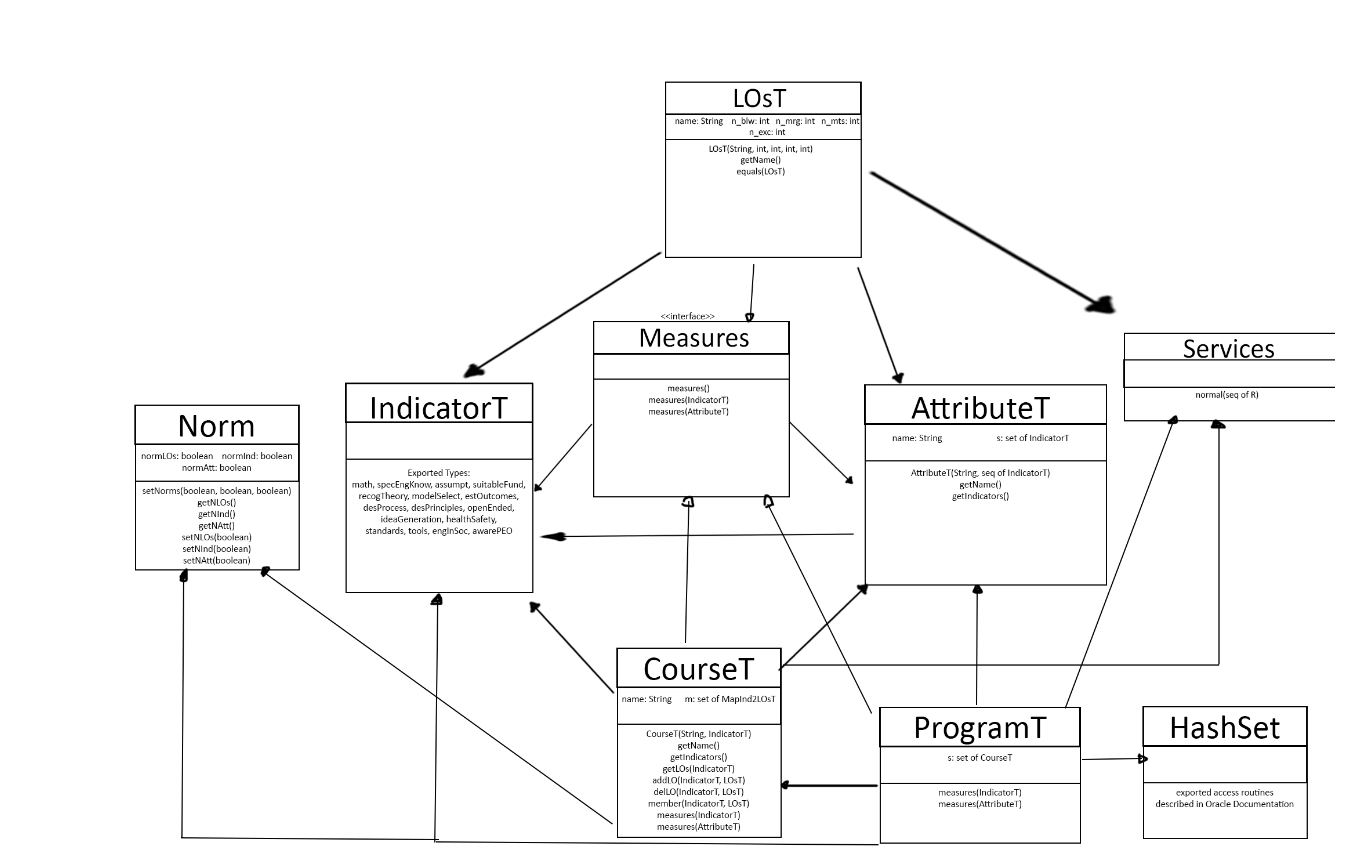
\includegraphics[width=1\textwidth]{images/uml_a3.png}
  \end{center}
  \item Draw a control flow graph for the convex hull algorithm. The graph should follow the approach used by the Ghezzi et al. textbook. In particular, the code statements should be edges of the graph, not nodes. Code for the convex hull algorithm can be found at: https://startupnextdoor.com/computing-convex-hull-in-python/. To match the diagrams available from Ghezzi, replace the for loop in the code with a while loop.
  \begin{center}
  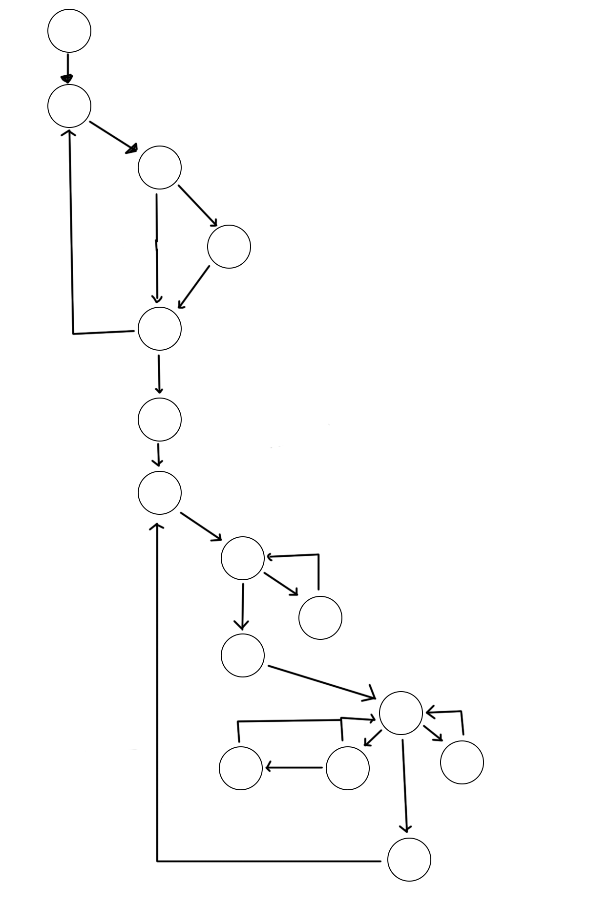
\includegraphics[width=0.7\textwidth]{images/control_flow.png}
  \end{center}
\end{enumerate}

\end {document}